\documentclass[a4paper,12pt]{article}

%% Language and font encodings
\usepackage[english]{babel}
\usepackage[utf8x]{inputenc}
\usepackage[T1]{fontenc}

%% Sets page size and margins
\usepackage[a4paper,top=3cm,bottom=2cm,left=3cm,right=3cm,marginparwidth=2 cm]{geometry}

%% Useful packages
\usepackage{amsmath}
\usepackage{graphicx}
\usepackage[colorinlistoftodos]{todonotes}
\usepackage[colorlinks=true, allcolors=blue]{hyperref}
\begin{document}
\begin{titlepage}
\begin{center}
		{\Large \textbf{Ludwig-Maximilians-Universität München}} \\
	\vspace{35mm}
{\bfseries\LARGE{Factor Immobility and Regional Impacts of Trade Liberalization: Evidence on Poverty from India}} \\{\bfseries\large{by Petia Topalova}} 
			\vspace{10mm}\\
            {\Large Advanced Seminar in Empirical International Trade } \\
			\vspace{2mm}
            {\Large{Bakai Baiazbekov
		\renewcommand\thefootnote{*}\footnote{B.Baiazbekov@campus.lmu.de}}}\\
        {\today}	\\
		\vspace{8mm}
		\begin{figure}[h] 
        \begin{center}

\includegraphics[width=0.6\textwidth]{lmu_siegel.png} \
\end{center}
\end{figure}%
	\end{center}

\end{titlepage}


\pagenumbering{Roman}
\setcounter{page}{2}
\tableofcontents  
\newpage



\pagenumbering{arabic}
\setcounter{page}{1}
\newpage
\section{Introduction}
The second half of the twentieth century witnessed one of the greatest increases in trade openness in the history of the world. Significant declines in tariffs and transportation costs have caused international trade to affect the economy of approximately every country. The theory and studies suggest that trade liberalization increases overall welfare, reasonable evidence on how trade liberalization affects distribution  and promotes free trade. \cite{NBERw12885} Free trade allows countries to trade goods without regulatory barriers or their associated costs. This decreases costs for countries that trade with other nations and may, ultimately, result in lower consumer costs because imports are subject to lower fees and there is increased competition. 

Trade liberalization increases competition from abroad, which might provide an incentive for greater efficiency and cheaper production by domestic firms. It might also act as an incentive for an economy to shift resources to industries they may have a competitive advantage in.  
This paper uses the 1991 Indian trade liberalization to measure the impact of trade liberalization on poverty, and to examine the mechanisms that support this impact. Generally speaking, trade liberalization is the removal or reduction of restrictions or barriers on the free exchange of goods between nations. This includes the removal or reduction of tariff obstacles, such as duties and surcharges, and non-tariff obstacles, such as licensing rules, quotas and other requirements.
\\ Variation in sectoral composition across districts and liberalization intensity across production sectors allows a difference - in - difference approach. Mostly, paper describes rural districts, where production sectors more exposed to liberalization were concentrated, experienced slower decline in poverty and lower consumption growth. 
Standard economic theory (i.e., the Heckshcer - Ohlin model) provides the prediction that with perfect \textbf{factor immobility}, gains to trade flow to the abundant factors, such as unskilled labor in developing countries. This findings from the recent trade models showed that the trade liberalization could reduce the wages of unskilled labor even in a labor abundant country, thereby shrinking the gap between the rich and the poor. \cite{Stiglitz70} For example, Abhijit B. and Andrew N. develop a model in which the short -run costs of factor reallocation following trade liberalization fall unequally on the poor.    
\\ This paper examines the effect of trade liberalization on poverty in India using the sudden and extensive change in India's trade policy in 1991. First of all, author reassess evidence initially presented in \cite{Topalova10}, districts more exposed to trade liberalization through their employment mix experienced slower progress in poverty reduction. Following, this paper extends that analysis by including nontariff barriers (NTBs) and by measuring how loss of trade protection affected consumption of households across the entire income distribution. Author, showed that finding is robust to a variety of approaches to deal with the potential endogeneity of the pre-liberalization composition and the confounding effect of concurrent reforms, including the break up of NTBs. The second contribution was about to explore the mechanisms by which \textbf{trade reform} may affect the income distribution, including factor mobility and adjustment in price levels. By identification strategy, developed in Topalova (2007), there was demonstrated that short -run adjustment costs of trade reforms influenced the schooling decisions of children. This paper establishes whether changes in district level poverty and levels of consumption across the income distribution before and after the trade reform are related to the reduction of trade protection at the district level. Difference -in -difference approach measures the relative effect of liberalization on districts that were more or less exposed to trade. 
\\ Author finds that the average real per capita expenditure in districts where employment was concentrated in industries exposed to larger tariff cuts grew relatively more slowly. 
This paper demonstrates the importance of factor mobility, and institutions that may affect it, in mitigating the unequal effects of trade liberalization. However, in states with flexible labor laws, movements of capital and labor across sectors and the overall faster growth of manufacturing eased the shock of relative price change. Finally, paper concludes that the adjustment to the trade reform came through changes in prices. Wages and wage premia seem to have absorbed the effect of the trade-induced relative price change. The inability of labor to reallocate away from sectors that lost trade protection is the most likely explanation for the observed relationship between trade liberalization and poverty in India's rural districts.  
\\ \textbf{Data} : The data was drawn from different sources: The rounds of the NSS regions provide information on household expenditure, occupation, industrial affiliation and individual statistics. This sample is approximately 75 000 rural and 45 000 urban households per round, where there are roughly 450 districts and 77 regions in India. Author, calculates district and region level measures of poverty and average consumption for 16 major Indian states for urban and rural populations.   

\textit{In conclusion : }This paper examined the evidence of the effect of India's opening to international trade in 1991 on poverty and consumption growth.  While poverty declined dramatically in both rural and urban in the 1990s,  rural areas in which employment was concentrated in sectors exposed to larger reductions in tariff protection experienced substantially less poverty reduction, and slower consumption growth than unexposed rural areas. The results are robust across a range of alternative specifications, including controlling for NTBs and other concurrent reforms. On average, a rural district experiencing no change in tariffs experienced a 14 percentage point decline in poverty.  In a district exposed to the average level of tariff reductions, poverty incidence declined by 11 - 12 percentage points. The impact on average consumption is much smaller. Correspondingly to rural districts which were not exposed to tariff cuts, districts with the average exposure to trade opening experienced approximately 3-4 percentage point lower consumption growth. The consumption growth of the poorest was hit disproportionately.  The findings of an effect of trade reform on poverty and consumption is consistent with a specific factor model of trade, in which labor is specific in the short run. Indeed, there was  very little evidence of trade-induced reallocation of workers both across geographical districts as well as across production sectors. The trade - consumption link is the strongest among those that are the least geographically mobile. Moreover,  Indian states with inflexible labor laws, where reallocation of labor across sectors and overall manufacturing growth may have been cut off, are precisely the areas where the adverse impact of trade opening on poverty was felt the most.  Some factors returns were affected by changes in relative output prices as a result  of trade reform.  
Overall, this paper concludes that  trade liberalization has strikingly heterogeneous effects, with different areas and segments of the population experiencing markedly different gains (or losses) than other segments depending on their ability to reallocate.  

\section{Main Part}

\subsection{Empirical Framework}
The Indian trade liberalization was sudden and externally imposed, providing an unusual natural experiment. Because the geographic location of production sectors  across the 450 Indian districts varied in 1991, the sudden removal of trade protection affected each district with a different intensity through the employment channel. It is thus possible to identify the impact of liberalization on poverty and consumption across the income distribution by comparing the evolution of these outcomes before and after the reforms in districts in which production sectors faced greater tariff cuts to districts in which production sectors remained relatively protected. 
\\Author, to measure a district's exposure to trade protection prior to liberalization  , calculates the average tariff faced by district as the nominal tariffs of the production sectors operating in that district as of 1991, by assigning to each production sector weight equal to the number of workers in that sector as a share of all workers in the district. The variation in the composition of production sector a weight equal to the number of workers in that sector as a share of all workers in the district. The Framework for regression model was as follows : 

\begin{equation}
\centering
Y_{dt} = \alpha + \beta_1 Tariff_{dt} + Post_t + \sigma_d + \epsilon_{dt}
\end{equation}

where $Y_{dt}$ is district level outcome, \textbf{poverty}; and $Tariff_{dt}$ is the level of protection by the district; $\beta$ is the coefficient of interest, that captures the average effect of trade protection on district outcomes; $\sigma_d$ is the inclusion of district fixed effects that controls for time -invariant heterogeneity at the district level, while year fixed effect; $Post_t$ controls for macroeconomic shocks or trends that affect India as whole. Author describes that this approach seeks to measure short to medium term effects of trade liberalization by comparing more exposed districts to less exposed districts. Equation (1) serves as a test of hypothesis of perfect factor mobility. For instance, if workers shift across districts in response to changes in wages and prices, the estimated effect $\beta$ would be zero. Moreover, he shows that, in fact, migration across districts plays no distinguishable role in Indian labor markets. Another advantage of this identification strategy is that it includes the general equilibrium effect of trade liberalization within geographical unit. The difference between previous studies have focused on the effect of trade opening on manufacturing workers, who, in developing countries, typically represent a small fraction of the population, though often a large share of income. This strategy captures not only the effect of trade liberalization on manufacturing and agricultural workers, but also on their dependents, and individuals in related and unrelated sectors. Trade liberalization affects individuals as consumers, and as a wage earners. \cite{Guido06} The empirical strategy employed in this paper focuses primarily on the effect of trade on the income earner, without explicitly modeling the effect of changes in prices of final goods.


\subsection{Measurement of Regional Exposure to Trade Liberalization}

In Table 1 was provided a summary statistics of the variables included in the analysis at the district level, including a breakdown of the workers across broad production sectors. From the table, the median district in India in 1991 had a population of approximately 22 million. In rural areas, approximately 80 percent of workers were involved in agriculture, where 87 percent were involved in the cultivation of cereals and oilseeds. Approximately 6 percent were involved in mining and manufacturing, while the remaining 12 percent worked in services, trade, transportation and construction. However, in urban India, agricultural employment is much lower, approximately 19 percent, while manufacturing and mining take 19 percent. And half of urban workers are either in service or in trade sectors. Following formula is provided for district tariffs: 

\begin{equation}
\centering
Tariff_{dt} = \frac{{\sum_i Worker_d,_i,1991} Tariff_i,_t}{Total Worker_d,1991}
\end{equation}

Nontraded industries , such as : services, trade, transport and cultivation of cereals and oilseeds, are assigned a zero tariff for the entire period. Since the identification strategies exploit change in tariffs within a district before and after the reform, it doesn't matter whether nontraded production sectors are assigned to zero or infinite tariffs as long as these tariffs do not change over time. For instances, \textbf{mean reversion} shows that poorer districts, which have a larger share of agricultural workers, may experience greater declines in poverty. This kind of districts will also record a lower decrease in tariffs, since the initial $Tariff_{dt}$ measure is low. A negative estimate of $\beta$ may not necessarily imply liberalization led to relative increases in poverty. Another possibility is that workers in traded and nontraded production sectors are on different growth paths. To solve it, author implemented $TrTariff_{dt}$ with $TrTariff_{dt}$ defined as : 

\begin{equation}
\centering
TrTariff_{dt} = \frac{{\sum_i Worker_d,_i,1991} Tariff_i,_t}{Total Worker_d,1991}
\end{equation}

$TrTariff_{dt}$ is nonscaled tariffs, ignores the workers in the nontraded production sectors. 


Another possible instrument was proposed that tariff changes are linearly related to initial tariffs. Tariff harmonization is one of the important reform goals, where it means that the higher the initial tariff, the greater tariff cut. One of the possible solutions would be to use the initial level of the scaled tariff interacted with a post dummy as an instrument. From previous, author argued that the scaled tariff measure is correlated with the \textit{pre-reform} levels of district income and poverty, and may thus not form a valid instrument. That's why he used a \textit{pre-reform} unscaled  tariff times a post dummy, in addition to the unscaled tariff, as instruments for tariff: 

\begin{equation}
\centering
Tariff_{dt} = \alpha + \beta_1 TrTariff_{dt} + \theta * Post_t * TrTariff_{d,1987} + Post_t + \sigma_d + \epsilon_{dt}
\end{equation}

In table 2, columns 2 and 4 shows the interaction of the initial unscaled tariff and a post -liberalization dummy. The interaction term is strongly correlated with the scaled tariff and adds explanatory power in all rural subsamples, through is less useful in urban sectors. 

\subsection{Mechanisms}

\textit{Reallocation across Regions :} In this paper was described the two basic trade models that demonstrate the link between factor prices and product prices. The very finding of regionally disparate effects of liberalization suggests the absence of perfect factor mobility across regions in India. In H-O model one would expect labor to mitigate in response to wage and price shocks, equalizing the incidence of poverty across regions. However, actual levels of migration in India contrast sharply with the assumptions of standard trade model. The pattern of migration has also remained remarkably constant through time, with no visible increase after the economic reforms of 1991. 

In table 1 demonstrated estimates of migration for rural and urban India based on two time periods, 1987 and 1999.  When we look to Panel A, rural, the overall migration is not low than 23 percent and 33 percent of urban residents have changed location of residence at least once in their lifetime.  However, from the results, most migrants are woman relocating at marriage, nearly 40 percent of females in rural and urban areas comparing with men's results 7 percent in rural and 26 percent in urban locations. Since the study was for short - run movement in past 10 years , only 3 to 4 percent of people living in rural areas reported changing either district or sector within past 10 years.  The figures shows that the percentage of women relocating is double the share of men. For people living in the urban areas the percentage of migrants is substantially higher. 

\begin{table}[h]
\centering
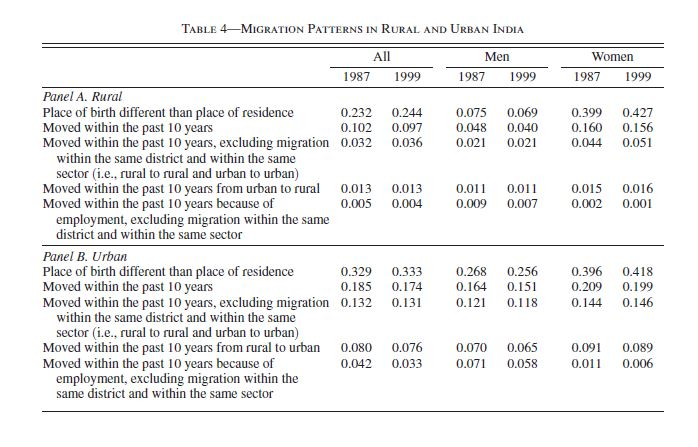
\includegraphics[width=1\textwidth]{table4.JPG}
\caption{\label{fig:Figure1}}
\end{table}

In table 2 author estimated the equations (4) , where the dependent variable is the share of in-migrants from outside district /sector.  Paper focuses on migrants who report to have relocated to the current district within the past ten years. While overall geographic mobility is low, there is substantial variation across different kinds of workers. For instance, skilled workers are much more likely to be in-migrants than workers without any education. Men who are in the top tenth percentile of the consumption distribution are four or five times more likely to be in-migrant than men who are in the bottom tenth percentile.  

To estimate the relationship between district tariffs and per capita consumption along the income distribution, author computed the tenth, twentieth, fortieth, sixtieth, eightieth, and ninetieth percentile of the consumption distribution, which are then used
as the outcome variables in specification (4). For more coherence, there is additional table 8, that demonstrates that one would expect the impact of the loss of trade protection to be felt most strongly among those that are the least mobile. The table presents , robustness, the results from estimating equation (4), allowing for time - varying effects of initial district characteristics.  The estimated effect of tariff cuts on log of per capita consumption is the largest for the households in the bottom tenth and twentieth percentile of the consumption distribution.  Generally speaking, as one moves up the income distribution, the effect decreases in magnitude and becomes statistically insignificant.  The estimate point for tariff effect declines from 1.5 to 0.1 from the top tenth percentile. 

\begin{table}[h]
\centering
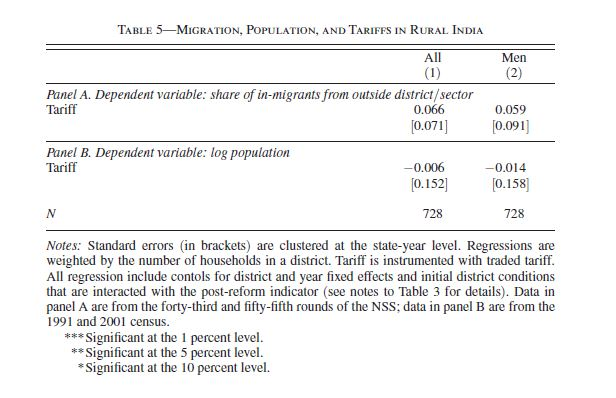
\includegraphics[width=1\textwidth]{table5.JPG}
\caption{\label{fig:Figure1}}
\end{table}

\textit{Reallocation across Production Sectors : }  There is a high levels of reallocation within districts, across production sectors, even if there is little migration across districts.  In this paper, author  examines whether the evidence from India supports the mechanism of adjustment suggested by the H-O:  a contraction of the sectors that experienced a decline in their output price, tariff reduction, and an expansion of those that experienced a relative price increase.  In figure 1 demonstrated the evolution of the three variables over time. There is no evidence of increase in job reallocation post 1991. Indeed, the measures of excess reallocation and structural change decline until 1996. Consistent with the findings  of low structural reallocation, employment shares remained remarkably constant.  Moreover, in paper \cite{Currie1997}, found relationship between trade liberalization and intersectoral  reallocation. In fact, these show that adjustment occurred through changes in relative wages. 

\textit{Trade liberalization and Institutional Characteristics  : }  to examine whether the institutionally driven mobility of labor across sectors underlies the poverty - trade liberalization link, author estimated equation (4) but allow for the effect of tariff cuts to vary according to the state's labor laws.  Trade liberalization had an effect on poverty and per capita expenditures predominantly in states with less flexible labor laws. The interaction between the tariff measure and the indicator of whether the district is in a state with flexible labor laws is of the opposite sign as the non - interacted tariff measure and of roughly the same magnitude, suggesting that the tariff cuts had no impact on poverty and consumption in states with flexible labor laws. 

\textit{Trade Liberalization and Factor Returns : } In this final statement, author discussed whether prices and factor returns adjusted in response to liberalization, i.e changes in domestic prices, factor returns, industry premia and agricultural wages.  Firstly, she evidenced that the tariff cuts indeed resulted in changes in domestic prices by using disaggregated data on the roughly 350 products that are included in India's whole sale price index during the 1987 - 2001 period, and regresses the log of the product prices on the lagged tariff of the product including year and product fixed effects. In table 9, was demonstrated a significant pass through of tariff changes to domestic prices like as the larger the tariff cut, the lower the price faced by domestic producers. Next, author showed the evidence that factor returns adjusted to the change in trade policy.  By constructing a measure of industry real wage as average payments per production worker, then regressing the log of this wage measure on lagged industry tariffs and industry and year dummies for the period 1988 - 1997. For instance, a 10 percent drop in tariffs leads to 0,8 percent decrease in industry wages.  Though these findings are indicative of the effect of reduced tariffs on industry specific returns, they omit important factors, such as the composition of the industrial labor force, which could drive this correlation. When producers faced with lower output prices, they might choose to substitute unskilled for skilled labor, without any change in relative wages, which would lead to a correlation between industrial wages and tariffs similar to what is in the data.  





\subsection{Main Findings}
One of the main findings is the estimation of the effect of liberalization on poverty and average consumption in rural and urban area. Below this text will be provided a two Tables, which represents each column reports a different version of equation. Shortly, Column 1 gives the OLS relationship with $Tariff_{dt}$. Column 2 reports the reduced form using $TrTariff_{dt}$. Column 3 is the Instrumental Variable(IV) approach using the $TrTariff_{dt}$ as an instrument for $Tariff_{dt}$. The regressions are weighted by the number of the households used to construct the estimate, to obtain a representative effect for rural and urban area and because of dependent variable is an estimate. The post-liberalization dummy $(Post_t)$ controls for macroeconomic shocks and time trends that affect India as whole, while the district fixed effects absorb district -specific heterogeneity. Author, clustered the standard errors at the state level, since the sectoral composition and economic growth may be correlated with in a state. Panel A shows the present results for poverty rate, while panel B gives the estimate for the log of the average per capita consumption in the district. These specification shows the significant relationship between reduction on the trade protection and relative increase in poverty in rural India.

I may see that the OLS point estimate is \textit{-0.24} but increases to \textit{-0.71 }, one percent level significancy when $TrTariff_{dt}$ is used as an instrument for $Tariff_{dt}$. In other words, this means that the cut in tariffs caused a relative poverty increase of about 3.9 percentage points in a district experiencing the average decline in scaled tariffs of 5.5 percentage points.  So, in this case for urban India, I see it doesn't make sense to make trade liberalization to positively effect poverty rate. For instance,  when I run the regression with Instrumented variable, the results showed no change \textit{-0.141} but approximately same, \textit{-0.169} on reduced reports. While the OLS relationship between changes in tariff measure and log consumption is negative in the rural India, the sign is reversed in the reduced form and IV specifications.  Larger drops in scaled tariffs corresponded to larger increases in the mean consumption. In rural sample, the basic results are robust to controlling for the time varying effect of district initial characteristics. The estimated relationship between tariffs and poverty rate falls from 0.71 to 0.47. Therefore, be the case that some of the variation in poverty incidence that equation (1) attributed to trade liberalization was due to certain omitted time - varying district specific characteristics. 

Next, I made regression and robustness check on urban area, The OLS estimates nearly same as in rural, \textit{-0.221} but with no significancy and it increases to \textit{-0.600} with one significant level.  In urban sample, including district initial characteristics drastically increases the magnitude of the estimated relationships for both dependent variables, though they remain rather imprecisely estimated. 

\begin{table}[h]
\centering
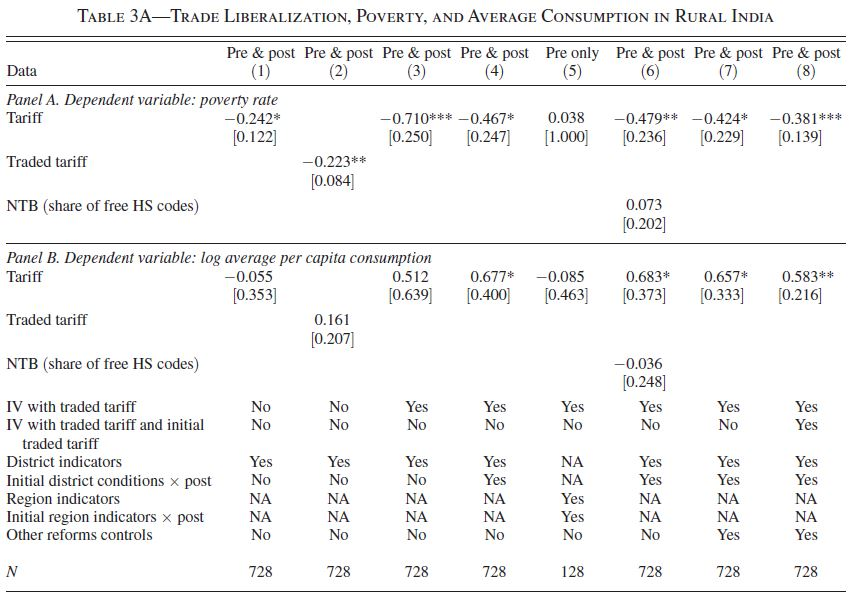
\includegraphics[width=1\textwidth]{Table3a.JPG}
\caption{\label{fig:Figure1}}
\end{table}

Now lets see what happens in urban area, where analysis can only be performed at the regional level, the point estimates of the effect of  tariff cuts on poverty are of similar size. Author tells that with fewer observations, estimation is less precise and the coefficients are not statistically distinguishable from zero (Table 2). In panel B, where the dependent variable: log average per capita consumption, author estimated the relationship between tariff reductions and per capita expenditure in the district. Nevertheless, the relationship is statistically significant only in Instrumental Variable specification, the estimated coefficient on the tariff measure from the OLS, reduced form and Instrumental Variable specification clearly demonstrate the biases that the OLS may introduce. From previous example, the OLS relationship between changes in tariff measure and log consumption is negative in rural India, the sign is reversed in the reduced form and Instrumental Variable specifications. The OLS relationship between in column 1 implies that the trade liberalization is associated with faster growth at the district level. Basically, larger drops in scaled tariffs correspond to larger increases in the mean consumption. However, the greater the share of workers involved in traded goods production sectors, the larger the drops in scaled tariffs i.e the more industrialized and richer is district. 

\begin{table}[h]
\centering
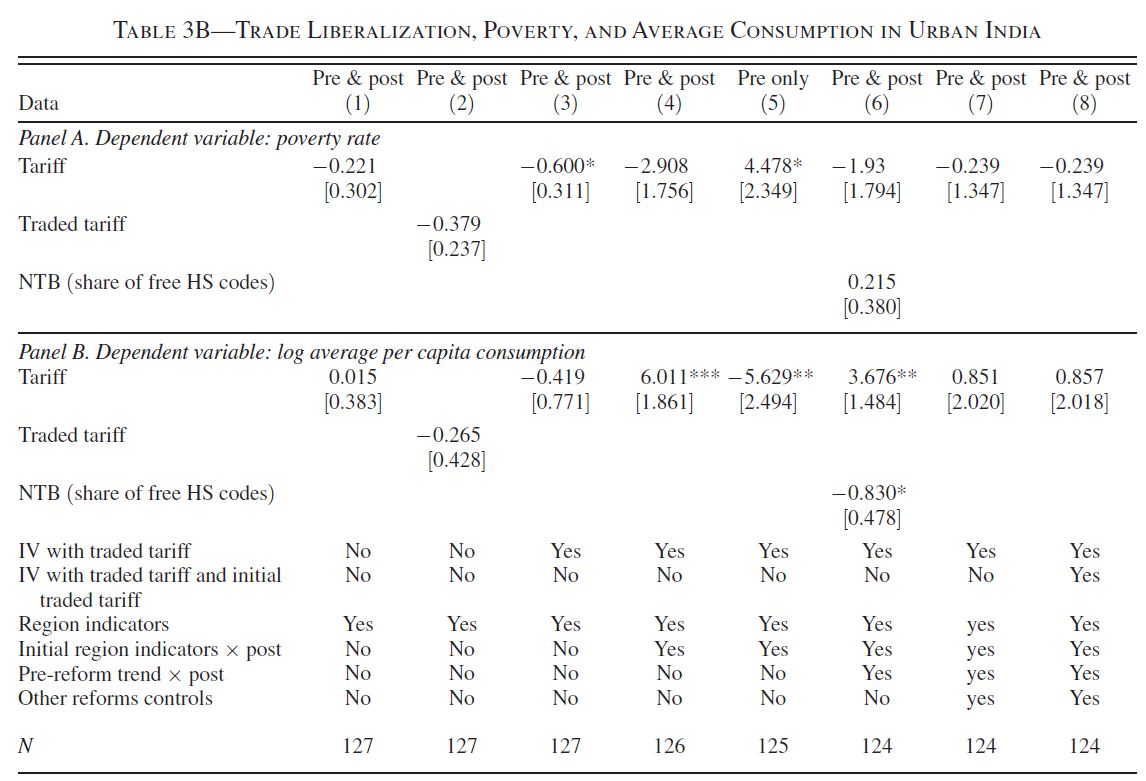
\includegraphics[width=1\textwidth]{table3b.JPG}
\caption{\label{fig:Figure1}}
\end{table}


An important point with specification in equation (1) is that changes in district trade protection, as captured in $Tariff$ and $TrTariff$, maybe systematically correlated with unobserved district-specific, time - varying shocks that affect the evolution of poverty or average consumption. If the initial sectoral composition or other pre - reform district characteristics have a bearing on the future growth in a district, the estimates in column 3 may be biased. As they are constrained by the very small number of states and they do not allow for initial state characteristics to have a time - varying effect \cite{Hasan07} .   Author reestimates equation (1) but allowing  initial 1987 district characteristics to have time - varying effect by interacting these with a post dummy: 

\begin{equation}
\centering
Y_{dt} = \alpha + \beta_1 Tariff_{dt} + \theta * Post_t * X_{d,1987} + Post_t + \sigma_d + \epsilon_{dt}
\end{equation}



The pre-reform characteristics $X_{d,1987}$, that are interacted with the post-liberalization dummy include the district's employment composition at a more aggregate level than the one used in the construction of the tariffs. In rural sample case, the results are robust to controlling for the time - varying effect of district initial characteristics (Column 4). The estimated relationship between tariffs and poverty rate falls from 0.71 to 0.47. Author states that it may be the case that some of variation in poverty incidence that equation (1) attributed to trade liberalization was due to certain omitted time - varying district specific characteristics. In urban case, including district initial characteristics drastically increases the magnitude of the estimated relationships for both dependent variables. There is a strong correlation between the pre - existing trends in outcome variables and trade liberalization shock at the region level in urban areas as demonstrated below. 

\subsection{Robustness}

The important matter of difference - in - difference estimates is possibility that pre - existing trends are correlated with changes in the variable of interest. Author makes a falsification test, to check if the measures of liberalization are correlated with district - level trends in poverty or consumption, whether changes in poverty or average consumption from 1983 to 1987 are correlated with changes in tariffs from 1987 to 1997. If the tariff drops are correlated with pre - existing trends in poverty and consumption, the coefficients on tariff should be similar to those estimated with the actual pre - and post - reform data. 

***In column 5 of both tables present the falsification exercise, which assigns the pre-reform tariffs(1987) to the 38 round and post - reform tariffs to the 43 round of data. 
There is no evidence, in rural sample, that the measure of trade liberalization is correlated with the pre - existing trends in the outcome variables. The estimated value of $\beta$ from the falsification regressions are very small in magnitude and of opposite sign compared to those in column 4. However, in urban sample, there exist strong correlation between the pre - reform poverty declines and consumption growth and tariff reduction. Particularly, faster growing regions in the 1980s experienced larger tariff cuts in the 1990s. Another important part of India's 1991 trade liberalization was the removal of NTBs. Author included the employment - weighted district or region measure of NTB in equation (4), in order to test whether the inclusion of measures of NTBs in their state - level analysis of the trade liberalization - poverty link in India drives the difference in the results.   

In column 6 was demonstrated that the point estimate and statistical significance of the effect of tariff cuts on poverty and consumption are invariant to the inclusion of NTBs. In contrast to the paper \cite{Hasan07}, the statistically insignificant coefficients on the NTBs suggest that the removal of these barriers to trade was associated with relative increase in poverty and relatively slower consumption growth in rural areas. Lastly, she tests other reforms, delicensed numerous industries after 1991 and eased restrictions on foreign direct investment, occuring at the same time as liberalization 

In column 7, she estimates the equation (4) including these time - varying district - level measures of reforms. The effect of trade liberalization on poverty and consumption in rural areas is insensitive to additional controls. However, in urban sample, the coefficient on the tariff measure declines substantially in magnitude once the controls for other reforms are included. This follows the higher concentration of manufacturing sectors in urban areas, which were also more affected by the opening of industries to foreign direct investment(FDI) and industrial delicensing. It replicates this more complete specification but instrument the scaled tariff with both unscaled tariff, $TrTariff$ , and their initial level interacted with a post liberalization indicator as described in equation (3). All findings are robust to this alternative instrumentation. 

As illustrated in table 1 and table 2, the point estimates on the tariff measures are more consistent across specifications, and more precisely estimated in the rural sample. On the other hand, in rural sample the coefficients are sensitive to the inclusion of various controls and are much less precisely estimated.  The effect is stronger in rural areas than in urban areas may at first appear ambiguous, as the concentration of workers in traded  sectors is higher in urban areas. However, there could several different reasons such as: poverty is much more common in rural India and density of households close to the poverty line is higher. The same negative income shock may have a larger impact on the poverty rate.  Next is the agricultural reforms were also an important component of the liberalization of 1991. The tariffs of agricultural products fell in line  with tariffs of manufacturing and other goods. While quantitative restrictions and licensing requirements on both the import and export of agricultural products  were removed later than on other goods, the share of agricultural products that could be freely imported jumped from 7 percent in 1989 to 40 percent in 1998. Author, runs a regression between agricultural tariffs and tariffs for mining and manufacturing . From the results, it is not surprisingly to sees that manufacturing workers are generally richer than agricultural workers and a decline in wages may not push them below the poverty line.  Final one focuses on the most demanding specification, in column 7, the significance of the estimated coefficients  in the urban and rural sample are of the same order. Because of smaller number of observations and the fact that in urban areas the regional change in tariffs, the noisiness of the urban estimates maybe very highly correlated with the pre-existing trends in the outcome variables and other reforms (Column 5). When allowing for the pre - existing trends to have time - varying effect and controlling effect for other reforms reduces the point estimates on the region tariff. However, there is still preventions of the possibility that tariff measure is capturing the effects of other time - varying regional shocks that have an effect on consumption growth and poverty in urban area. Since the urban results were substantially noisier, paper was concentrated mainly on the findings of rural India. 

Until now, this paper has established that, whatever the effects of trade liberalization were, rural areas with employment concentrated in sectors that were disproportionately affected by trade liberalization, experienced slower growth in average consumption and slower progress in poverty reduction.    








\newpage
\bibliographystyle{alpha}
\bibliography{sample}

\newpage
\section{Statutory Declaration}
I declare that I have authored this thesis independently, that I have not used other than the declared sources / resources, and that I have explicitly marked all material which has been quoted either literally or by content from the used sources.

\newpage
\section{Appendix}
\begin{table}[h]
\centering
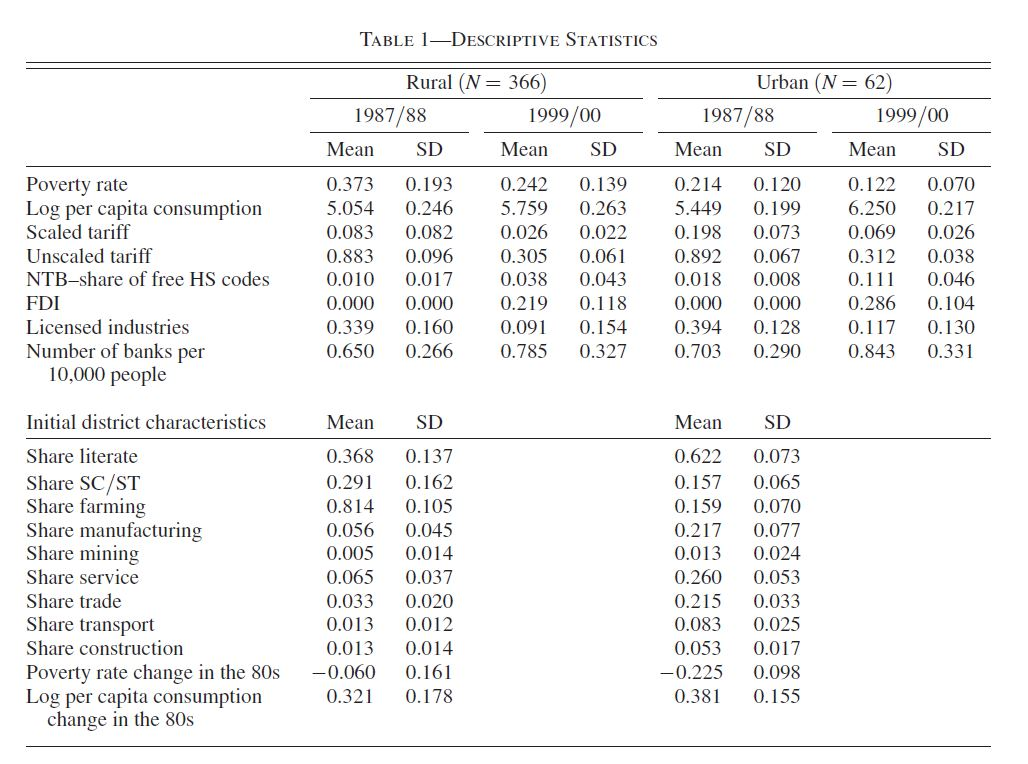
\includegraphics[width=1\textwidth]{Tbale1.JPG}
\caption{\label{fig:Figure1}}
\end{table}

\begin{table}[h]
\centering
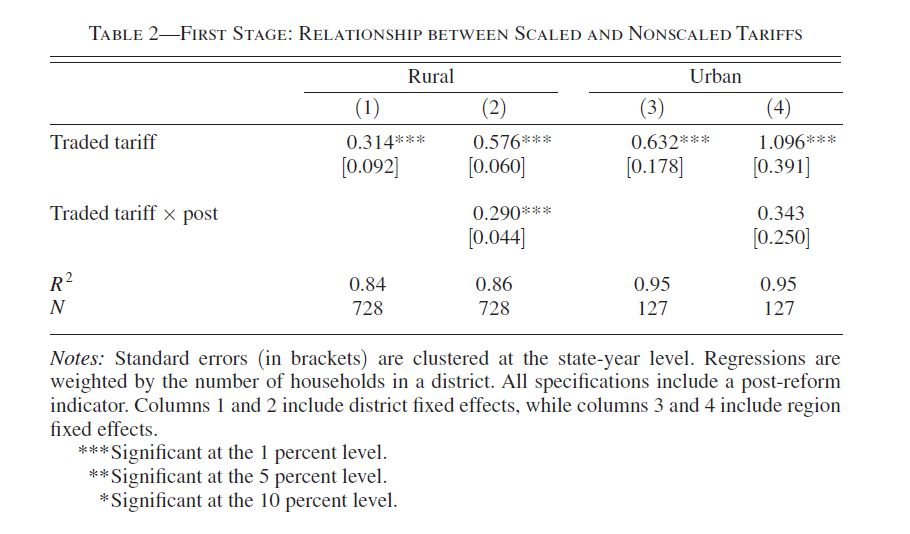
\includegraphics[width=1\textwidth]{table2.JPG}
\caption{\label{fig:Figure1}}
\end{table}

\begin{table}[h]
\centering
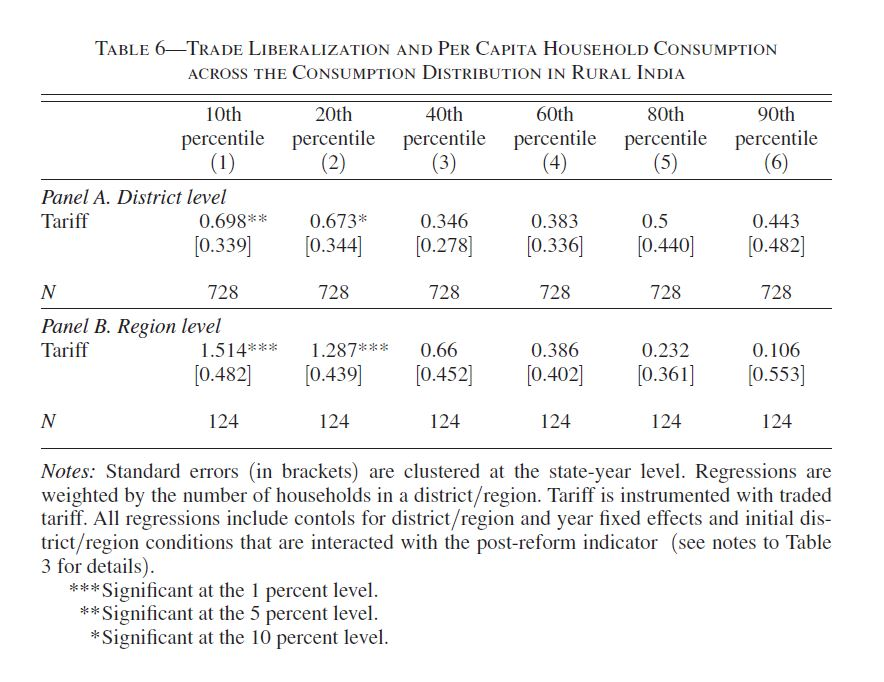
\includegraphics[width=1\textwidth]{table6.JPG}
\caption{\label{fig:Figure1}}
\end{table}

\begin{table}[h]
\centering
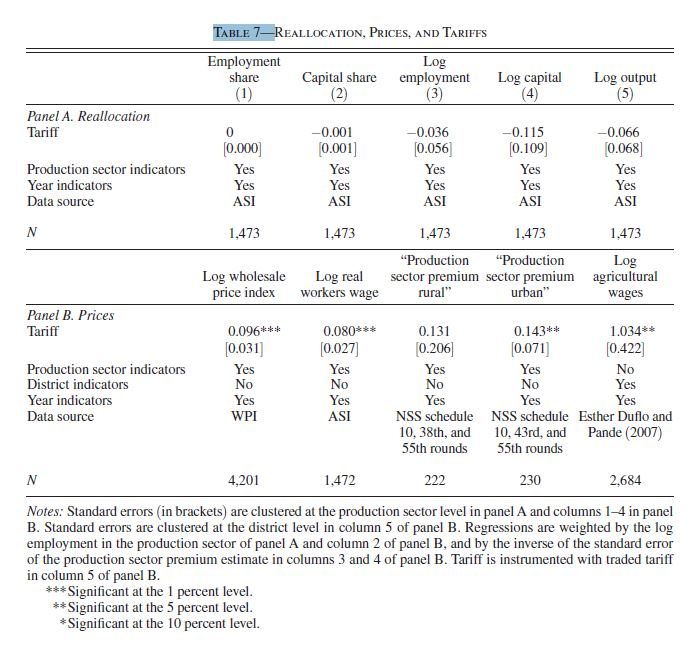
\includegraphics[width=1\textwidth]{table7.JPG}
\caption{\label{fig:Figure1}}
\end{table}

\begin{table}[h]
\centering
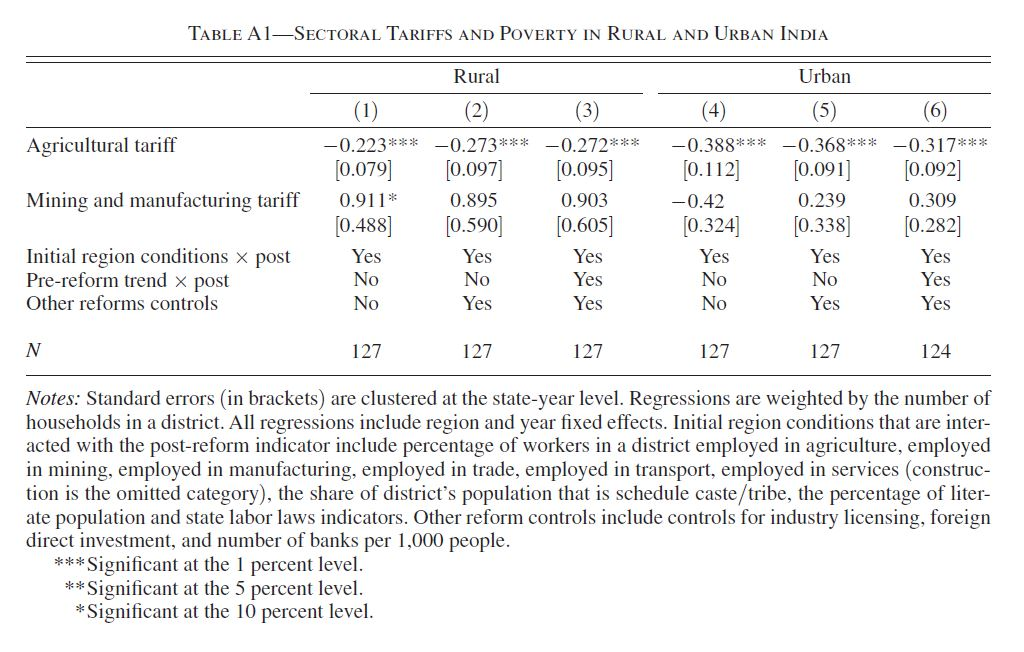
\includegraphics[width=1\textwidth]{table1Appendix.JPG}
\caption{\label{fig:Figure1}}
\end{table}

\begin{figure}[h]
\centering
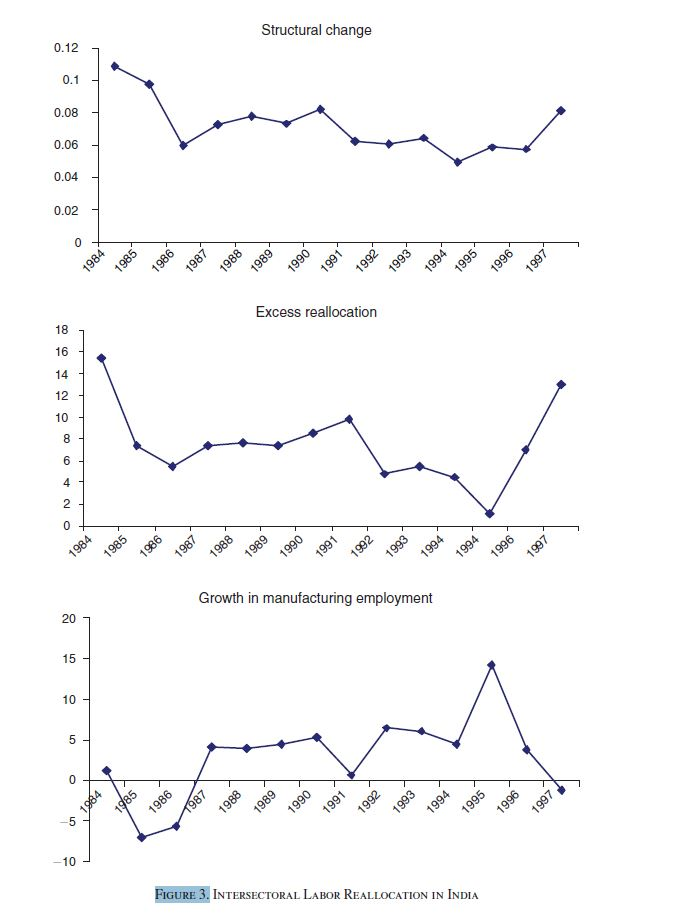
\includegraphics[width=1\textwidth]{fig3.JPG}
\caption{\label{fig:Figure1}}
\end{figure}
\end{document}
\end{document}